\documentclass[12pt, onecolumn, a4paper]{article}
\usepackage[a4paper, margin=1.15in]{geometry}
\usepackage[hidelinks]{hyperref} 
\usepackage{graphicx}       
\usepackage{epsfig, subfigure, amsthm, amsmath, amssymb} 
\usepackage{xcolor}
\usepackage[numbers]{natbib} % اضافه کردن بسته مدیریت مراجع  
\usepackage{setspace}       
\usepackage{tikz}           
\usepackage{enumitem}       
\usepackage{pifont}          
\usepackage[extrafootnotefeatures]{xepersian} 
\settextfont[Scale=1.2]{BZAR.TTF} 
\setlatintextfont[Scale=1]{Times New Roman} 
\usepackage[bottom]{footmisc} 


\setlength{\parindent}{2em} % فرورفتگی ابتدای پاراگراف
\setlength{\parskip}{0.5em} % فاصله بین پاراگراف‌ها
\linespread{1.5} % فاصله بین خطوط
\setlist[itemize]{label=$\bullet$, leftmargin=1.5em, itemsep=0.5em}

% تعریف اعداد فارسی برای متن رفرنس‌ها
\renewenvironment{abstract}{%
	\noindent\textbf{\large چکیده}\[0.5em]%
	\noindent\ignorespaces%
}{%
	\par\noindent%
}


\begin{document}
	
	\title{بهینه‌سازی خوشه‌بندی و مسیریابی در شبکه‌های حسگر بی‌سیم با مدل‌های \lr{IMD-EACBR}، \lr{EECHS-ISSADE} و \lr{ABC-ACO}} 
	\author{فائزه قیاسی، رانیا کارگر، ملیکا ملکی\\
		دانشجویان کارشناسی دانشگاه صنعتی اصفهان\\
		مهندسی کامپیوتر}
	\date{}
	\maketitle
	\thispagestyle{empty}
	\vfill
	
	\section*{چکیده}
	شبکه‌های حسگر بی‌سیم و اینترنت اشیا به دلیل کاربردهای گسترده در زمینه‌هایی مانند نظارت محیطی، حمل‌ونقل هوشمند و مراقبت‌های بهداشتی، اهمیت زیادی پیدا کرده‌اند. یکی از چالش‌های اصلی این شبکه‌ها، محدودیت انرژی گره‌های حسگر است که بر طول عمر شبکه تأثیر می‌گذارد. برای حل این مشکل، استفاده از تکنیک‌های مسیریابی مبتنی بر خوشه‌بندی همراه با الگوریتم‌های فراابتکاری برای انتخاب سرخوشه‌ها و طراحی مسیرهای بهینه‌ی انتقال داده‌ها پیشنهاد شده است. در این مقاله، سه مدل به‌منظور بهینه‌سازی مصرف انرژی و بهبود عملکرد شبکه ارائه می‌شوند. مدل \lr{IMD-EACBR} که از الگوریتم ارشمیدس بهبودیافته برای انتخاب سرخوشه‌ها و از الگوریتم بهینه‌سازی مبتنی‌بر آموزش و یادگیری اصلاح‌شده برای مسیریابی چندپرشی استفاده می‌کند، مدل \lr{EECHS-ISSADE} که ترکیبی از الگوریتم‌های جست‌وجوی گنجشک و تکامل تفاضلی را برای خوشه‌بندی و مسیریابی پیشنهاد می‌دهد و مدل \lr{ABC-ACO} که از الگوریتم زنبورعسل مصنوعی و کلونی مورچه‌ها برای کاهش تأخیر و توازن مصرف انرژی بهره می‌برد. نتایج شبیه‌سازی نشان می‌دهد که مدل‌های پیشنهادی در مقایسه با روش‌های قبلی، طول عمر شبکه را افزایش داده، مصرف انرژی را کاهش می‌دهند و نرخ انتقال داده‌ها را بهبود می‌بخشند. 
	
	\newpage
	
	\section{مقدمه}
	در سال‌های اخیر، اینترنت اشیا\LTRfootnote{Internet Of Things} و شبکه‌های حسگر بی‌سیم\LTRfootnote{Wireless Sensor Networks} به عنوان دو فناوری نوین و کلیدی، نقش مهمی در زمینه‌های مختلفی از جمله نظارت بر محیط، مراقبت‌های بهداشتی هوشمند، حمل‌ونقل هوشمند و اتوماسیون صنعتی ایفا کرده‌اند \cite{ref1, ref2, ref3}. در این شبکه‌ها، گره‌های حسگر\LTRfootnote{Sensor Nodes} به‌صورت گسترده در مناطق جغرافیایی پراکنده می‌شوند. این گره‌ها اطلاعات محیطی را جمع‌آوری کرده و به ایستگاه پایه\LTRfootnote{Base Station} ارسال می‌کنند که در شکل \ref{fig:your_label} نمونه‌ای از آن را مشاهده می‌کنید. یکی از چالش‌های اصلی این شبکه‌ها، محدودیت انرژی گره‌های حسگر است، زیرا این گره‌ها معمولاً وابسته به باتری‌های محدود هستند. مصرف سریع انرژی در گره‌ها می‌تواند باعث کاهش طول عمر شبکه\LTRfootnote{Network Lifetime} و اختلال در انتقال داده‌ها شود. به همین دلیل، بهینه‌سازی مصرف انرژی و طراحی راهکارهایی برای افزایش طول عمر شبکه از مهم‌ترین اولویت‌ها در این حوزه به شمار می‌روند.
	
	\begin{figure}[h]
		\centering
		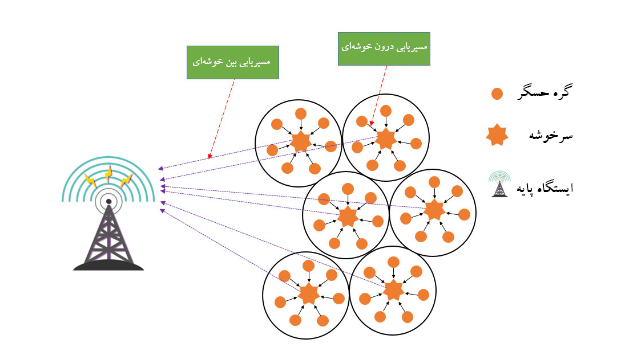
\includegraphics[width=\textwidth]{cluster-persian.png}
		\caption{یک شبکه حسگر بی‌سیم خوشه‌ای}
		\label{fig:your_label}
	\end{figure}
	
	یکی از راهکارهای مؤثر برای مقابله با محدودیت‌های انرژی در شبکه‌های حسگر بی‌سیم، استفاده از تکنیک‌های مسیریابی مبتنی بر خوشه‌بندی است. در این روش، شبکه به چندین خوشه تقسیم می‌شود و برای هر خوشه یک سرخوشه\LTRfootnote{Cluster Head} تعیین می‌گردد. سرخوشه‌ها مسئول جمع‌آوری داده‌ها از گره‌های عضو خوشه و انتقال آن‌ها به ایستگاه پایه هستند. انتخاب بهینه سرخوشه‌ها و مسیریابی داده‌ها\LTRfootnote{Data Routing} به منظور کاهش مصرف انرژی، افزایش طول عمر شبکه و بهبود کارایی، به‌ویژه در شبکه‌های بزرگ و پیچیده، اهمیت زیادی دارد.
	
	برای انتخاب بهینه سرخوشه‌ها، الگوریتم‌های فراابتکاری\LTRfootnote{Metaheuristic Algorithms} متعددی ارائه شده‌اند. این الگوریتم‌ها با استفاده از روش‌های بهینه‌سازی پیشرفته و تحلیل پارامترهای مرتبط، نقش مهمی در کاهش مصرف انرژی و افزایش طول عمر شبکه ایفا می‌کنند. برخی از الگوریتم‌های مؤثر در این زمینه عبارتند از:
	
	\begin{itemize}
		\item \textbf{الگوریتم بهینه‌سازی ارشمیدس بهبودیافته}\LTRfootnote{Improved Archimedes Optimization Algorithm}:  الگوریتم ارشمیدس بهبودیافته با بهره‌گیری از یک تابع تناسب\LTRfootnote{Fitness Function} که پارامترهایی نظیر فاصله، بهره‌وری انرژی و درجه گره را در نظر می‌گیرد، سرخوشه‌های بهینه را انتخاب می‌کند.
		\item \textbf{الگوریتم جست‌وجوی گنجشک}\LTRfootnote{Sparrow Search Algorithm}: این الگوریتم از رفتار اجتماعی گنجشک‌ها در یافتن منابع غذایی الهام گرفته و با تحلیل انرژی باقی‌مانده گره‌ها و فاصله آن‌ها از ایستگاه پایه، سرخوشه‌های بهینه را تعیین می‌کند.
		\item \textbf{الگوریتم تکامل تفاضلی}\LTRfootnote{Differential Evolution}: الگوریتم  تکامل تفاضلی با بهره‌گیری از روش‌های بهینه‌سازی با پیچیدگی کم و پایدار، فرآیند انتخاب سرخوشه‌ها را تسهیل می‌کند.
		\item \textbf{الگوریتم زنبورعسل بهبودیافته}\LTRfootnote{Improved Artificial Bee Colony}: الگوریتم زنبورعسل بهبود یافته با الهام از رفتار زنبورها در یافتن منابع غذایی، گره‌هایی با بیشترین بهره‌وری انرژی و مناسب‌ترین موقعیت مکانی را به عنوان سرخوشه انتخاب می‌کند.
	\end{itemize}
	
	علاوه بر انتخاب سرخوشه‌ها، طراحی الگوریتم‌های بهینه برای مسیریابی داده‌ها از دیگر چالش‌های اساسی در شبکه‌های حسگر بی‌سیم است. این الگوریتم‌ها با هدف کاهش مصرف انرژی، بهبود تأخیر در انتقال داده‌ها و افزایش کارایی طراحی می‌شوند. برخی از الگوریتم‌های برجسته در این زمینه شامل موارد زیر است:
	
	\begin{itemize}
		\item \textbf{الگوریتم مسیریابی چندپرشی مبتنی بر بهینه‌سازی آموزش و یادگیری اصلاح‌شده‌ی ترکیبی}\LTRfootnote{Teaching-learning-Based Optimization for Multi-Hop Routing}: الگوریتم مسیریابی چندپرشی از روش‌های بهینه‌سازی مبتنی بر آموزش و یادگیری برای یافتن مسیرهای بهینه بین گره‌ها استفاده می‌کند.
		\item \textbf{الگوریتم کلونی مورچه بهبودیافته}: الگوریتم کلونی مورچه بهبودیافته با ایجاد مسیرهای چندپرشی بهینه از سرخوشه‌ها به ایستگاه پایه، به کاهش مصرف انرژی کمک می‌کند.
	\end{itemize}
	
	این مقاله تلاش دارد تا با طراحی و بررسی مدل‌های پیشنهادی، گام‌های مؤثری در راستای کاهش مصرف انرژی، افزایش طول عمر شبکه و بهبود عملکرد اینترنت اشیا و شبکه‌های حسگر بی‌سیم بردارد.
	
	
\section{کارهای مرتبط}

در سال‌های اخیر، تحقیقات گسترده‌ای برای بهینه‌سازی خوشه‌بندی و مسیریابی در شبکه‌های حسگر بی‌سیم صورت گرفته است. در این بخش به مرور برخی از مهم‌ترین پژوهش‌های انجام‌شده پرداخته می‌شود:

\begin{itemize}
	\item \textbf{پروتکل \lr{LEACH}}: یکی از نخستین روش‌های خوشه‌بندی است که به‌طور گسترده استفاده شده است \cite{ref1, ref5}. این پروتکل سرخوشه‌ها را به صورت تصادفی انتخاب می‌کند و از مسیریابی تک‌مرحله‌ای استفاده می‌کند. با این حال، این روش در شبکه‌های بزرگ‌تر به دلیل مصرف بالای انرژی ناکارآمد است.
	
	\item \textbf{پروتکل‌های مبتنی بر الگوریتم‌های فراابتکاری}: الگوریتم‌هایی مانند \lr{PSO} و \lr{ABC} برای بهبود مصرف انرژی معرفی شده‌اند \cite{ref4, ref6}. این الگوریتم‌ها با در نظر گرفتن فاکتورهایی مانند انرژی باقی‌مانده گره‌ها و فاصله تا ایستگاه پایه، سرخوشه‌های بهینه را انتخاب می‌کنند.
	
	\item \textbf{پروتکل‌های ترکیبی}: در پژوهش‌هایی مانند \cite{ref5, ref7}، ترکیب الگوریتم‌های مختلف از جمله جستجوی گنجشک و زنبورعسل باعث بهبود طول عمر شبکه و کاهش تأخیر شده است.
	
	\item \textbf{روش‌های جدید مبتنی بر یادگیری ماشینی}: برخی پژوهش‌ها از مدل‌های یادگیری ماشینی مانند شبکه‌های عصبی و یادگیری تقویتی برای پیش‌بینی مسیرهای بهینه استفاده کرده‌اند \cite{ref8, ref9}.
\end{itemize}

	
	این مرور نشان می‌دهد که پژوهش‌های انجام‌شده پیشرفت‌های قابل‌توجهی در بهینه‌سازی خوشه‌بندی و مسیریابی ارائه داده‌اند. با این حال، همچنان نیاز به توسعه روش‌های کارآمدتر با قابلیت انطباق بیشتر در سناریوهای پویای اینترنت اشیا وجود دارد.
\newpage
	
\section{روش‌شناسی}

در این بخش، سه مدل پیشنهادی \lr{IMD-EACBR}، \lr{EECHS-ISSADE} و \lr{ABC-ACO} با الگوریتم‌های مرتبط برای خوشه‌بندی و مسیریابی تشریح می‌شوند. هدف اصلی این مدل‌ها افزایش کارایی انرژی، کاهش تأخیر، و بهبود طول عمر شبکه در شبکه‌های حسگر بی‌سیم است.

\subsection{مدل \lr{IMD-EACBR}}
مدل \lr{IMD-EACBR} یک روش خوشه‌بندی و مسیریابی مبتنی بر فراابتکاری برای شبکه‌های حسگر بی‌سیم است که از الگوریتم بهینه‌سازی ارشمیدس بهبودیافته برای انتخاب سرخوشه‌ها بهره می‌برد \cite{ref4, ref5}. این مدل با طراحی توابع هدف بهینه‌سازی، کارایی انرژی و طول عمر شبکه را افزایش می‌دهد.

\subsubsection{مرحله خوشه‌بندی}
خوشه‌بندی یکی از مراحل کلیدی این مدل است که با استفاده از الگوریتم ارشمیدس انجام می‌شود. هدف این مرحله، کاهش مصرف انرژی در انتقال داده‌ها از گره‌های حسگر به ایستگاه پایه است. تابع هدف برای انتخاب سرخوشه‌ها به صورت زیر تعریف می‌شود:

\begin{equation}
	F = \alpha \times E_r + \beta \times D_{ch} + \gamma \times N_{degree}
\end{equation}

در اینجا:
\begin{itemize}
	\item $E_r$ انرژی باقی‌مانده گره‌ها است.
	\item $D_{ch}$ فاصله میان گره‌ها و سرخوشه است.
	\item $N_{degree}$ تعداد گره‌های عضو خوشه است.
	\item $\alpha$، $\beta$ و $\gamma$ ضرایب وزنی هستند که اهمیت هر پارامتر را مشخص می‌کنند.
\end{itemize}

این فرمول با هدف تعادل انرژی و کاهش فاصله انتقال طراحی شده است.

\subsubsection{مرحله مسیریابی}
در این مدل، مسیریابی چندمرحله‌ای با استفاده از الگوریتم \lr{TLBO} انجام می‌شود. این الگوریتم مسیرهایی با حداقل مصرف انرژی و تأخیر را شناسایی می‌کند. انرژی مصرفی برای انتقال داده‌ها به صورت زیر محاسبه می‌شود:

\begin{equation}
	E_{total} = \sum_{i=1}^{N} \left( E_{tx}(d_{i}) + E_{rx} \right)
\end{equation}

که در آن:
\begin{itemize}
	\item $E_{tx}(d_{i})$ انرژی مورد نیاز برای ارسال داده با فاصله $d_{i}$ است.
	\item $E_{rx}$ انرژی مورد نیاز برای دریافت داده است.
	\item $N$ تعداد گره‌های درگیر در انتقال داده است.
\end{itemize}

\subsection{مدل \lr{EECHS-ISSADE}}
مدل \lr{EECHS-ISSADE} ترکیبی از الگوریتم‌های جستجوی گنجشک و تکامل تفاضلی برای انتخاب سرخوشه‌ها و مسیریابی ارائه می‌دهد \cite{ref5, ref6}. این مدل به طور خاص برای شبکه‌های حسگر بی‌سیم بزرگ طراحی شده است و تلاش می‌کند تا با به حداقل رساندن فاصله خوشه‌ها و استفاده از الگوریتم‌های بهینه‌سازی چندهدفه، مصرف انرژی را کاهش دهد.

\subsubsection{الگوریتم جستجوی گنجشک}
این الگوریتم با الهام از رفتار اجتماعی گنجشک‌ها، سرخوشه‌ها را بر اساس انرژی باقی‌مانده و فاصله از ایستگاه پایه انتخاب می‌کند. تابع هدف برای این الگوریتم به صورت زیر تعریف می‌شود:

\begin{equation}
	F_{sparrow} = \sum_{i=1}^{N} \left( \frac{E_i}{D_i} \right)
\end{equation}

در اینجا:
\begin{itemize}
	\item $E_i$ انرژی باقی‌مانده گره $i$.
	\item $D_i$ فاصله گره $i$ از ایستگاه پایه.
	\item $N$ تعداد گره‌ها در خوشه است.
\end{itemize}

\subsubsection{الگوریتم تکامل تفاضلی}
الگوریتم تکامل تفاضلی برای جلوگیری از همگرایی زودهنگام استفاده می‌شود و تنوع جمعیت در انتخاب سرخوشه‌ها را تضمین می‌کند. این الگوریتم به خصوص در شبکه‌های حسگر بی‌سیم با توزیع متراکم گره‌ها مؤثر است.

\subsection{مدل \lr{ABC-ACO}}
مدل \lr{ABC-ACO} یک روش خوشه‌بندی و مسیریابی است که از الگوریتم زنبورعسل مصنوعی بهبودیافته برای انتخاب سرخوشه‌ها و الگوریتم کلونی مورچه برای یافتن مسیرهای بهینه استفاده می‌کند \cite{ref6, ref7}.

\subsubsection{الگوریتم زنبورعسل مصنوعی}
این الگوریتم با شبیه‌سازی رفتار زنبورهای عسل، سرخوشه‌هایی با انرژی بیشتر و فاصله کمتر از ایستگاه پایه را انتخاب می‌کند. تابع هدف آن به صورت زیر تعریف شده است:

\begin{equation}
	F_{ABC} = \frac{E_r}{D_{ch}}
\end{equation}

\subsubsection{الگوریتم کلونی مورچه}
برای یافتن مسیرهای بهینه از الگوریتم کلونی مورچه استفاده می‌شود. فرمول بهینه‌سازی مسیرها در این الگوریتم به صورت زیر است:

\begin{equation}
	P_{ij} = \frac{\tau_{ij}^\alpha \cdot \eta_{ij}^\beta}{\sum_{k \in N} \tau_{ik}^\alpha \cdot \eta_{ik}^\beta}
\end{equation}

در اینجا:
\begin{itemize}
	\item $\tau_{ij}$ میزان فرومون مسیر $i$ به $j$.
	\item $\eta_{ij}$ معکوس فاصله مسیر $i$ به $j$.
	\item $\alpha$ و $\beta$ وزن‌های فرومون و فاصله هستند.
\end{itemize}

\begin{figure}[h]
	\centering
	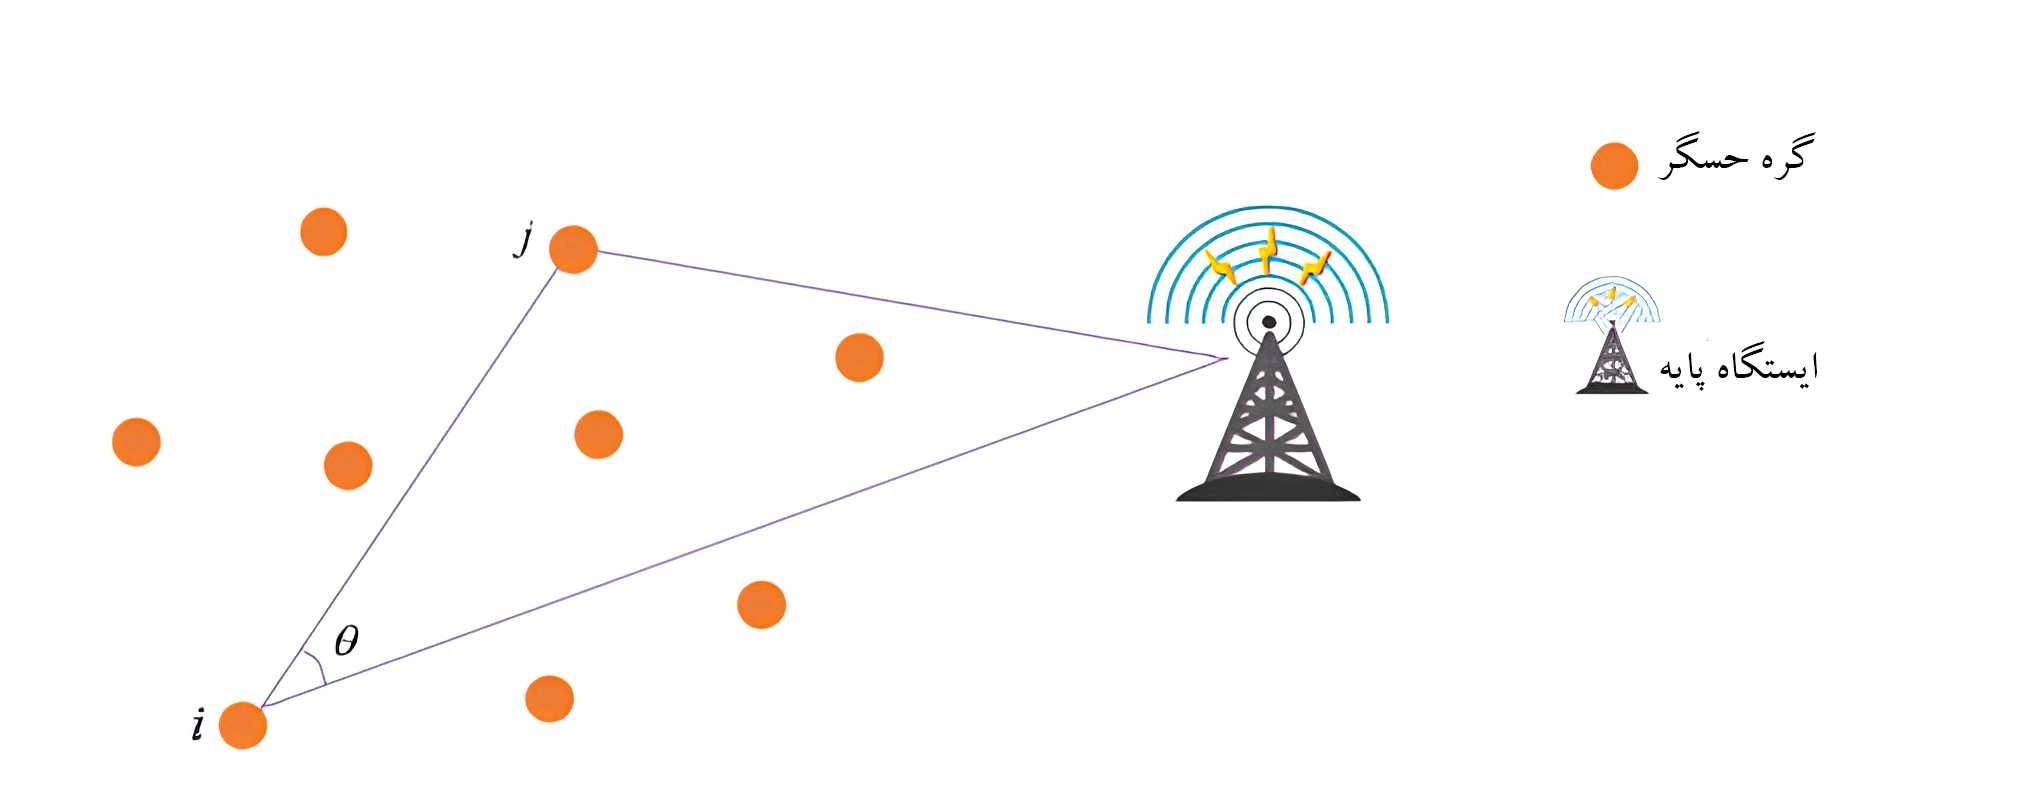
\includegraphics[width=0.8\textwidth]{routing-abc-aco.png}
	\caption{نمای کلی مسیریابی در مدل \lr{ABC-ACO}}
	\label{fig:routing_abc_aco}
\end{figure}

شبیه‌سازی‌ها نشان داده‌اند که این مدل می‌تواند طول عمر شبکه را به طور قابل توجهی افزایش داده و بهره‌وری انرژی را بهبود بخشد.

\section{نتایج و تحلیل}

نتایج شبیه‌سازی با استفاده از نرم‌افزار \lr{MATLAB} انجام شده و عملکرد سه مدل پیشنهادی با روش‌های موجود مقایسه شده است. معیارهای ارزیابی شامل طول عمر شبکه، مصرف انرژی، نرخ انتقال داده، و نسبت تحویل بسته بوده‌اند. 

جدول \ref{table:results} مقایسه عملکرد مدل‌های پیشنهادی را ارائه می‌دهد. همان‌طور که مشاهده می‌شود، هر یک از مدل‌ها در برخی جنبه‌ها نسبت به سایرین برتری دارد. 

\begin{table}[h!]
	\centering
	\caption{مقایسه عملکرد مدل‌های پیشنهادی}
	\label{table:results}
	\resizebox{1\textwidth}{!}{ % تنظیم عرض جدول به 100 درصد عرض صفحه
		\begin{tabular}{|c|c|c|c|c|}
			\hline
			\textbf{مدل} & \textbf{طول عمر شبکه (دور)} & \textbf{مصرف انرژی (ژول)} & \textbf{نرخ انتقال داده (بسته/ثانیه)} & \textbf{نسبت تحویل بسته (\%)} \\ \hline
			\lr{IMD-EACBR} & 3500 & 0/047 & 0/975 & 98/83 \\\hline
			\lr{EECHS-ISSADE} & 3250 & 0/056 & 0/945 & 97/62 \\\hline
			\lr{ABC-ACO} & 3100 & 0/063 & 0/910 & 96/45 \\\hline
		\end{tabular}
	}
\end{table}

\subsection*{تحلیل طول عمر شبکه}
مدل \lr{IMD-EACBR} بیشترین طول عمر شبکه را ارائه داده است. این امر به دلیل توزیع متوازن بار میان سرخوشه‌ها و استفاده بهینه از انرژی گره‌ها است \cite{ref4, ref5}. همچنین، استفاده از الگوریتم ارشمیدس بهبودیافته برای انتخاب سرخوشه‌ها باعث شده که این مدل بهره‌وری بالایی در مصرف انرژی داشته باشد. 

مدل \lr{EECHS-ISSADE} با طول عمر 3250 دور در رتبه دوم قرار دارد. ترکیب الگوریتم‌های جستجوی گنجشک و تکامل تفاضلی، توانسته است کارایی خوبی در مدیریت انرژی شبکه داشته باشد \cite{ref6}. با این حال، پیچیدگی‌های محاسباتی بیشتر این مدل نسبت به \lr{IMD-EACBR} ممکن است منجر به کاهش طول عمر آن شده باشد.

مدل \lr{ABC-ACO} با طول عمر 3100 دور در مقایسه با دو مدل دیگر عملکرد کمتری داشته است. دلیل این امر می‌تواند استفاده از الگوریتم کلونی مورچه باشد که هزینه محاسباتی بیشتری دارد و انرژی بیشتری مصرف می‌کند \cite{ref7}.

\subsection*{تحلیل مصرف انرژی}
از نظر مصرف انرژی، مدل \lr{IMD-EACBR} کمترین مصرف انرژی (0/047 ژول) را داشته است که نشان‌دهنده بهره‌وری بالا در انتقال داده‌ها و مدیریت خوشه‌بندی است. این موفقیت ناشی از بهینه‌سازی‌های چندهدفه در الگوریتم‌های استفاده‌شده در این مدل است.

مدل \lr{EECHS-ISSADE} نیز مصرف انرژی نسبتاً کمی (0/056 ژول) داشته است. استفاده از الگوریتم‌های جستجوی گنجشک و تکامل تفاضلی، نقش مهمی در کاهش مصرف انرژی ایفا کرده است \cite{ref5}.

مدل \lr{ABC-ACO} بیشترین مصرف انرژی (0/063 ژول) را داشته است. این موضوع به دلیل نیاز به به‌روزرسانی مداوم فرومون‌ها در الگوریتم کلونی مورچه است که مصرف انرژی بیشتری دارد \cite{ref6}.

\subsection*{تحلیل نرخ انتقال داده}
از نظر نرخ انتقال داده، مدل \lr{IMD-EACBR} با نرخ 0/975 بسته در ثانیه بهترین عملکرد را داشته است. این نرخ بالا ناشی از کاهش تأخیر در ارسال داده‌ها و انتخاب مسیرهای بهینه برای انتقال است.

مدل \lr{EECHS-ISSADE} با نرخ انتقال داده 0/945 بسته در ثانیه عملکرد قابل‌قبولی دارد. این عملکرد نشان می‌دهد که ترکیب الگوریتم‌های استفاده‌شده در این مدل توانسته است مسیرهای کارآمدی برای انتقال داده‌ها پیدا کند \cite{ref5}.

مدل \lr{ABC-ACO} با نرخ انتقال داده 0/910 بسته در ثانیه پایین‌ترین عملکرد را در میان سه مدل دارد. این امر به دلیل پیچیدگی مسیریابی در این مدل و زمان بیشتری است که برای پیدا کردن مسیرهای بهینه صرف می‌شود.

\subsection*{تحلیل نسبت تحویل بسته}
از نظر نسبت تحویل بسته، مدل \lr{IMD-EACBR} با نرخ 98/83\% بهترین عملکرد را دارد. این موفقیت ناشی از انتخاب دقیق سرخوشه‌ها و مسیرهای چندپرشی بهینه است.

مدل \lr{EECHS-ISSADE} با نرخ 97/62\% در جایگاه دوم قرار دارد. استفاده از الگوریتم‌های چندهدفه در این مدل به کاهش از دست رفتن بسته‌ها کمک کرده است \cite{ref6}.

مدل \lr{ABC-ACO} با نرخ 96/45\% کمترین عملکرد را داشته است. دلیل این امر می‌تواند به پیچیدگی‌های مسیریابی و کاهش بهره‌وری انرژی در این مدل مربوط باشد \cite{ref7}.

\section{بحث و تحلیل}

نتایج شبیه‌سازی نشان داد که مدل \lr{IMD-EACBR} با استفاده از الگوریتم ارشمیدس بهبودیافته و مسیریابی چندپرشی، عملکرد بهتری نسبت به مدل‌های دیگر دارد. این مدل به دلیل توزیع متوازن بار بین گره‌های شبکه، باعث افزایش طول عمر شبکه شده است. همچنین، مصرف انرژی در این مدل به میزان قابل‌توجهی کاهش یافته و نرخ انتقال داده بهبود پیدا کرده است. 

در مقایسه، مدل \lr{EECHS-ISSADE}، که از ترکیب الگوریتم‌های جستجوی گنجشک و تکامل تفاضلی استفاده می‌کند، در شبکه‌های بزرگ‌تر و پیچیده‌تر عملکرد مطلوبی داشته است. دلیل این امر، توانایی این مدل در جلوگیری از همگرایی زودهنگام و تضمین تنوع در فرآیند خوشه‌بندی و مسیریابی است. 

مدل \lr{ABC-ACO} نیز در کاهش تأخیر و بهبود نرخ انتقال داده موفق عمل کرده است. این مدل با استفاده از الگوریتم کلونی مورچه برای مسیریابی، توانسته است مسیرهای بهینه را برای ارسال داده‌ها پیدا کند. با این حال، مصرف انرژی در این مدل نسبت به دو مدل دیگر بیشتر بوده است که می‌تواند به دلیل ساختار پیچیده‌تر الگوریتم کلونی مورچه باشد.

با توجه به این تحلیل‌ها، می‌توان نتیجه گرفت که هر یک از مدل‌ها نقاط قوت و ضعف خاص خود را دارند و انتخاب مدل مناسب بستگی به شرایط و نیازهای خاص شبکه دارد.

\section{نتیجه‌گیری و پیشنهادات آینده}

در این مقاله، سه مدل پیشنهادی برای بهینه‌سازی خوشه‌بندی و مسیریابی در شبکه‌های حسگر بی‌سیم معرفی شدند. هر مدل با استفاده از الگوریتم‌های پیشرفته فراابتکاری، مصرف انرژی را کاهش داده و طول عمر شبکه را به میزان قابل‌توجهی افزایش می‌دهد. نتایج شبیه‌سازی نشان داد که مدل \lr{IMD-EACBR} به دلیل استفاده از الگوریتم ارشمیدس بهبودیافته و رویکرد چندپرشی، در مقایسه با سایر روش‌ها عملکرد بهتری از خود نشان داده است. مدل \lr{EECHS-ISSADE} نیز به واسطه ترکیب الگوریتم‌های جستجوی گنجشک و تکامل تفاضلی توانست در شبکه‌های بزرگ و پیچیده کارایی مطلوبی داشته باشد. همچنین، مدل \lr{ABC-ACO} با استفاده از الگوریتم زنبورعسل و کلونی مورچه، تأخیر در انتقال داده‌ها را کاهش داده و نرخ انتقال داده را بهبود بخشید.

\subsection*{دستاوردهای کلیدی}
\begin{itemize}
	\item افزایش طول عمر شبکه و کاهش مصرف انرژی در گره‌های حسگر.
	\item بهبود نرخ انتقال داده و کاهش تأخیر در انتقال اطلاعات.
	\item ارائه مدل‌هایی که قابل پیاده‌سازی در سناریوهای مختلف و مقیاس‌های بزرگ‌تر هستند.
\end{itemize}

\subsection*{پیشنهادات برای پژوهش‌های آینده}
\begin{enumerate}
	\item \textbf{به‌کارگیری روش‌های یادگیری عمیق:} ترکیب الگوریتم‌های فراابتکاری با شبکه‌های یادگیری عمیق برای پیش‌بینی بهتر الگوهای مصرف انرژی و بهبود تصمیم‌گیری در انتخاب سرخوشه‌ها.
	\item \textbf{بررسی تأثیر ایستگاه پایه متحرک:} گسترش مدل‌های پیشنهادی برای شبکه‌هایی که در آن‌ها ایستگاه پایه قابلیت حرکت دارد، به‌ویژه در سناریوهایی مانند پهپادهای متحرک.
	\item \textbf{افزودن معیارهای کیفی دیگر:} بررسی تأثیر عواملی نظیر قابلیت اطمینان ارتباط، امنیت داده‌ها، و تأخیر شبکه در مدل‌های پیشنهادی.
	\item\textbf{پیاده‌سازی در محیط‌های واقعی:} ارزیابی مدل‌ها در محیط‌های فیزیکی و مقایسه عملکرد آن‌ها با شبیه‌سازی‌های نرم‌افزاری.
	\item \textbf{بررسی تطبیق‌پذیری در اینترنت اشیا:} گسترش مدل‌ها برای سازگاری بهتر با سناریوهای متنوع اینترنت اشیا، شامل شبکه‌های هوشمند و صنعتی.
\end{enumerate}

نتایج این پژوهش نشان‌دهنده توانایی بالای مدل‌های پیشنهادی در افزایش بهره‌وری و کاهش هزینه‌های عملیاتی شبکه‌های حسگر بی‌سیم است. توسعه بیشتر این مدل‌ها می‌تواند گامی مؤثر در راستای ایجاد شبکه‌های پایدار و کارآمد در کاربردهای اینترنت اشیا باشد.

% References
\renewcommand{\bibname}{مراجع} % تغییر عنوان بخش مراجع به "مراجع"

\begin{thebibliography}{99}
	
	\begin{latin}
		
		\bibitem{ref1} \lr{Sharma, Deepak, and Amol P. Bhondekar. "Traffic and energy aware routing for heterogeneous wireless sensor networks." \textit{IEEE Communications Letters} 22.8 (2018): 1608-1611.}
		
		\bibitem{ref2} \lr{Farsi, Mohammed, et al. "A congestion-aware clustering and routing (CCR) protocol for mitigating congestion in WSN." \textit{IEEE Access} 7 (2019): 105402-105419.}
		
		\bibitem{ref3} \lr{Satpathy, Sambit, et al. "Design a FPGA, fuzzy based, insolent method for prediction of multi-diseases in rural area." \textit{Journal of Intelligent \& Fuzzy Systems} 37.5 (2019): 7039-7046.}
		
		\bibitem{ref4} \lr{Kathiroli, Panimalar, and Kanmani Selvadurai. "Energy efficient cluster head selection using improved Sparrow Search Algorithm in Wireless Sensor Networks." \textit{Journal of King Saud University-Computer and Information Sciences} 34.10 (2022): 8564-8575.}
		
		\bibitem{ref5} \lr{Lakshmanna, Kuruva, et al. "Improved metaheuristic-driven energy-aware cluster-based routing scheme for IoT-assisted wireless sensor networks." \textit{Sustainability} 14.13 (2022): 7712.}
		
		\bibitem{ref6} \lr{Wang, Zongshan, et al. "An energy efficient routing protocol based on improved artificial bee colony algorithm for wireless sensor networks." \textit{IEEE Access} 8 (2020): 133577-133596.}
		
		\bibitem{ref7} \lr{Mohan, Prakash, et al. "Improved metaheuristics-based clustering with multihop routing protocol for underwater wireless sensor networks." \textit{Sensors} 22.4 (2022): 1618.}
		
		\bibitem{ref8} \lr{Yue, Jiangyue, et al. "A hybrid optimization-based clustering algorithm for energy-efficient wireless sensor networks." \textit{IEEE Transactions on Industrial Informatics} 17.4 (2021): 2413-2424.}
		
		\bibitem{ref9} \lr{Chen, Shuo, et al. "Energy-efficient cluster head selection in wireless sensor networks with metaheuristic optimization." \textit{IEEE Sensors Journal} 20.23 (2020): 14012-14022.}
		
		\bibitem{ref10} \lr{Lyu, Xuan, et al. "Dynamic energy-aware clustering and routing algorithm for wireless sensor networks." \textit{Journal of Network and Computer Applications} 193 (2022): 103162.}
		
	\end{latin}
	
\end{thebibliography}


\end{document}
